\documentclass[oneside,openright,frontopenright, singlespacing]{dmathesis}
\input{preamble}
\usepackage{cite}
\usepackage{breqn}
\begin{document}
\title{Null geodesics}
\subtitle{Modelling light in the Kerr metric}
\author{Joseph A Sweeney}
\researchgroup{Mathematics}
\pagenumbering{roman}
\maketitlepage*

\begin{abstract}
%
	In this paper I will show and discuss my findings on numerical methods and optimisations for modelling solutions to the equations of motion derived from geodesic equations in the Schwarzschild and Kerr metric using Python. In the first section, I will introduce some key information and language associated with General Relativity, which this paper will rely upon. Then, I will demonstrate methods for modelling null (light-like) geodesics in a metric. Using these I will model various black holes as seen directly in front of an observer with any given celestial sphere.
%
\end{abstract}

\begin{declaration*}
%
	This piece of work is a result of my own work except where it forms an assessment based on group project work. In the case of a group project, the work has been prepared in collaboration with other members of the group. Material from the work of others not involved in the project has been acknowledged and quotations and paraphrases suitably indicated.
%
\end{declaration*}

\disableprotrusion
\tableofcontents*
\enableprotrusion

\cleardoublepage
\pagenumbering{arabic}

%\include{background}
%\include{paper1}
%\include{paper2}
%\include{paper3}
\begin{introduction}

	The field of black hole imaging in Physics and Computer Science had a wave of enthusiasm 
	and development following Christopher Nolan’s 2014 blockbuster Interstellar\cite{Interstellar}, and the imaging of the supermassive 
	black hole at the centre of M87 by the Event Horizon Telescope in 2019\cite{event2019first}. Producing high quality images 
	and videos of black holes and wormholes can be very computationally costly, so ingenious ways of gaining 
	efficacy are often used. My aim is to explore these methods and tricks to present practical approaches 
	to modelling the Schwarzschild metric and Kerr metric. After this I will explore accretion discs and gravitational redshift to create as realistic a model as possible.

\end{introduction}

\chapter{A brief history of modelling black holes}

	The history and development of black hole simulations is fascinating; the field was considered relatively useless untill the 90's, so progression was incrimental but crucial. In this chapter I will give you a rundown of some of the most important breakthroughs relevant to this paper, specifically work involving Schwarzschild and Kerr black holes.

\section{1915-1970: Theoretical}

	Our story begins in 1915 at the Prussian Academy of Sciences, where Albert Einstein presented his General Theory of Relativity\cite{einstein1915feldgleichungen} in a four part speech. One of the most significant developments in modern science; General Relativity allowed humans to think of gravity in an entirely new way, revolutionising large mass interactions.

\vspace{1em}
	Only one year later, Karl Schwarzschild published an exact solution to Einsteins Field equations\cite{schwarzschild1916gravitationsfeld}, this solution was named the Schwarzschild metric in honour of its discoverer and can be used to describe a non-rotating, non-charged black hole. Interestingly, only four months later Johannes Droste independently published a paper going into more detail with the same metric\cite{droste1917field}, which he discovered at a similar time to Schwarzschild.

\vspace{1em}
	Skipping significantly ahead in time, Roy Kerr published his solution to Einsteins Field equations, describing the space around a rotating, non-charged mass. This solution was published in 1963\cite{kerr1963gravitational}, after Kerr corrected a pre-print from Newman, Tambourino and Unti which claimed to prove the lack of existence of any meaningful rotating space\cite{newman1963empty}.

\vspace{1em}
	Following on from Kerr's work, Carter made an extensive anaysis of the Kerr metric in his paper Global Structure of the Kerr family of Gravitational Fields\cite{carter1968global}

\vspace{1em}
	Using the growing background of work that had been put into this field, Godfrey published a paper which was filled with inaccuracies, so is rarely cited; but in amongst these inaccuracies was the first correct prediction of the D-shaped of the shadow caused by a Kerr black hole with various spin parameters.

\section{1971-1990: Models begin}

	In 1972 James Bardeen began the first thorough study on the effects of gravitational lensing caused by Kerr black holes\cite{bardeen1973timelike}, working with his student C.T Cunningham, Bardeen published the paper "The optical appearance of a star orbiting an extreme Kerr black hole"\cite{cunningham1973optical} in which amongst other key things, Bardeen proposed the same D-shaped shadow as Godfrey, but is often cited as being the first. As well as this, the first figure of the primary and secondary images created by a light-source in a circular orbit in the equatorial plane was included; with position as seen by a distant observer plotted over time (see figure 1.1).

\begin{figure}[!ht]
	\centering
	\includegraphics[width=0.4\linewidth]{img/Cunningham-Bardeen-1973-2images-2}
	\caption{The path(s) of a lightsource in the Kerr metric. \cite{cunningham1973optical}}
\end{figure}

\vspace{1em}
	Cunningham released a paper in 1975 which presented the effects of redshift on an accretion disc in a Kerr black holes equatorial plane\cite{cunningham1975effects}, but did not include an image of such effects.

\vspace{1em}
	In 1978, Jean-Pierre Luminet publishes the first image of the effects of gravitational lensing caused by a Kerr black hole\cite{luminet1979image}. This image was actually hand drawn using ink but the intensity for each region had been calculated using numerical techniques. This image took into account the effect bolometric luminocity flux (change in brightness) and still stands as a remarkably accurate image for its time.

\begin{figure}[!ht]
	\centering
	\includegraphics[width=0.5\linewidth]{img/Luminet-drawing}
	\caption{The first 'image' of a Kerr black hole. \cite{luminet1979image}}
\end{figure}

\vspace{1em}
	In a paper by Fukue and Yokohama in 1988, the first non-bolometric coloured image of the same simulation as above was released\cite{fukue1988color}.

\section{1991-2022: Chasing realism}

	By 1990, the existence of black holes was all but confirmed, and the scientific community were in general agreement of there existence in the universe. This, coupled with more computational power lead to the field of black hole imaging becoming much more viable. In the era presented in this subchapter, far more than I could fit in has happened; but I present some of the key events.

\vspace{1em}
	Tragically given his untimely death at the age of 40, much of J.A Mark's work is unpublished and unreleased, but what we do know is that in 1993 he produced the first animation of an flight inside a Schwarzschild black hole, and a flight over an elliptical orbit\cite{InfinitelyCurved}.

\vspace{1em}
	At this stage more and more reallistic images could be generated, with the magneto-hydrodynamics of black holes being proposed by Bardeen, Carter and Hawking in 1972\cite{bardeen1973four} and computers being capable of handling more complex computiation.

\vspace{1em}
	One of the most realistic images generated of a Schwarzschild black hole without an accretion disc, and in fact one of the most realistic animations were produced by Alain Riazuelo (available online at \cite{riazuelo2014black}).

\vspace{1em}
	Of course the most significant recent events in black hole imagine occured in 2014 and 2019 respectively, with the release of the film Interstellar and the release of the images taken of the supermassive black hole M87. Along with the release of the film Interstellar came two papers \cite{thorne2015gravitational}\cite{thorne2015visualizing} which broke down the process for generating realistic images and animations of Kerr black holes and Ellis-Thorne wormholes. The Kerr black hole shown in the film is unrealistic, even though it was generated mathematically; this is due to artistic choices made by director Christopher Nolan, leading to the lack of accounting for the Doppler effect and changes in energy flux. See Figure 1.3 and 1.4 for the most realistic image generated by Thorne et al. and the final product which was used in the film.

\begin{figure}[!ht]
	\centering
	\begin{minipage}{0.5\textwidth}
		\centering
		\includegraphics[width=0.9\linewidth]{img/realistic-kerr}
		\caption{A very realistic model of a Kerr black hole. \cite{Interstellarpaper1}}
	\end{minipage}%
	\hfill
	\begin{minipage}{0.5\textwidth}
		\centering
		\includegraphics[width=0.9\linewidth]{img/used-kerr}
		\caption{A Kerr black hole as seen in Interstellar. Credit: DNeg and Warner Bros. Entertainment Inc.}
	\end{minipage}
\end{figure}

\vspace{1em}
	Finally, the successful imaging of supermassive black hole M87 using the worldwide event horizon telescope gave physical evidence as to the realism of previously generated images, and with that, evidence to support the validity of Einsteins General Theory of Relativity. Who knows how far humans will progress in this field, perhaps in the next 100 years we will have an image as high definition as the generated images presented above and throughout this paper of the black hole at the centre of the milkyway StrA*.

\vspace{1em}
	With the background of the field behind our backs, we can persevere into the maths and physics behind it all, and create some images similar to those which made history.


\chapter{Introduction to General Relativity}
	Albert Einstein’s theory of General Relativity is a pivotal achievement in the scientific community, and the field of General Relativity has revolutionised our understanding of the universe. Here I will introduce and summarise some key components and notation for ease of readers in later sections.

\section{Special relativity}

	A precursor to General relativity, Einsteins theory of special relativity started as a mostly algebraic field, with little geometric application. As time passed however the scientific community found that special relativity gives us a framework to view the universe in the absence of gravitational fields far more appropriate than anything before.

\vspace{1em}
	The idea of relativity predates Einstein quite substantially, the Galilean principle of relativity states the fundamental laws of physics are unchanged between frames of reference moving with constant velocity with respect to one another.

\vspace{1em}
	Einsteins special principle of relativity states\cite{}: "If a system of coordinates K is chosen so that, in relation to it, physical laws hold good in their simplest form, the same laws hold good in relation to any other system of coordinates K' moving in uniform translation relatively to K."

\vspace{1em}
	The theory of Special relativity is based upon the combination of this statement, and the postulate that the speed of light in a perfect vacuum is the same for any observer, independent of the light source and observers motion.

\vspace{1em}
	Although Newtonian mechanics work remarkably well at low velocities, they break down as we approach the speed of light. It is in these scenarios in which we turn to relativity to accurately describe and analyse systems. Many ideas and effects inferred by special relativity have been experimentally proved; such as the relativistic Doppler effect.

\vspace{1em}
	General relativity takes its name from the fact that it is a generalisation of special relativity, covering systems in which gravitational field are present. In this paper we will be using little from special relativity, other than mentioning relativistic abberation and Doppler shift (which can be described in special relativity more easily).

\section{Geodesics}

	In his theory of General Relativity, Einstein formalised gravity not as a force - as it is thought of in Newtonian physics - but as the curvature of spacetime. Spacetime is the 4-dimensional plane we exist in, one dimension representing time, and three space. 

\vspace{1em}
	The path of an object acted upon solely by gravity can be thought of as moving along curved spacetime, with the path being a straight line if the effects of gravity are non-existent. Such a path through curved spacetime is called a geodesic, and equations of motion in General Relativity are governed by constants derived from geodesic equations – which in turn are derived from the metric in which the object finds itself. 

\vspace{1em}
	The origins of considering curved spacetime come from Riemannian geometry, which is a form of differential geometry; the study of curvature and surfaces. Using the relatively pure field, we can take many properties and relations found and apply them to the curvature of spacetime.

\vspace{1em}
		We see in Figure 2.1 a common representation of the curvature of spacetime, this is actually an artists rendition of what is called an embedding diagram; since we are trying to visualise four dimensions as a plane we must embed our higher dimensional image such that spacetime is represented as a flat plane. We can then visualise to what extent bodies of mass affect the curvature of this plane. Naturally if there is any curvature it ceases to be a plane, but it is called as such because this is it's form under no gravitational effects.

\begin{figure}[!ht]
	\centering
	\includegraphics[width=0.5\linewidth]{img/curved-spacetime}
	\caption{A representation of curved spacetime}
\end{figure}

\vspace{1em}
	Above I mentioned the geodesic, and the way I introduced them was a simplification; the formal definition of a geodesic is the shortest path between two points on a surface. In general relativity geodesics fit into three catagories:

\vspace{1em}
\begin{itemize}
  \item Timelike geodesic - A timelike geodesic describes a test particle of non-zero mass $\Rightarrow$ travelling below the speed of light in a vaccum.
  \item Lightlike geodesic - A lightlike (or null) geodesic describes a test particle of zero mass $\Rightarrow$ travelling at the speed of light in a vaccum.
  \item Spacelike geodesic - Spacelike geodesics have little place in general relativity as they have no concrete physical representation. By some definitions they describe the path of a test particle travelling faster than the speed of light, and that will do for us.
\end{itemize}

\vspace{1em}
	 In this paper, a null-geodesic will always be describing the path of a photon in a metric. Geodesic equations can be thought of as a generalisation of Newton's second law of motion, taking into account the curvature of the spacetime one chooses. I.e instead of F = 0 $\Rightarrow$ a = 0, we have that F = 0 implies that acceleration is sufficient to keep the motion in a straight line when considered in Euclidean space.

\section{Metrics and conventions}

\vspace{1em}
	Metrics are sections of spacetime which are solutions to Einstein’s field equations, the equation that defines his General theory. As an example, the simplest solution to these field equations describing a black hole is the Schwarzschild metric. A metric is generally given in line notation - which informs one how a small change in spacetime relates to changes in the variables we consider the object to be moving in. The relation between geodesic equations and metrics are governed by Christoffel symbols, denoted $\Gamma$, seen in the below general form of a geodesic equation[pg. 156-157]\cite{schutz2009first}:  

	\[\frac{d^2 \gamma^\lambda}{dt^2} + {\Gamma^\lambda}_{\mu\nu} \frac{d\gamma^\mu}{dt} \frac{d\gamma^\nu}{dt} = 0\]

\vspace{1em}
	As is common in papers studying light and the astrological, I will be using natural units: That is, I will be taking c = G = 1, this results in non-SI units, but conversion is possible and generally simple. A distance of 1 will correspond to $1$(s) x c($ms^{-1}$) = the distance travelled by light in a vaccum in one second.

\vspace{1em}
	The celestial sphere from a point in space is an image of all the points taken to be arbitrarily far away - using the distance I take in this paper for earth; it is the sky in all directions excluding the moon, mercury and mars. (My 'arbitrary distance' is t=1000 i.e the distance light travels in a vaccum in 1000 seconds)

\vspace{1em}
	Christoffel symbols are incredibly important in the study of General Relativity, relating directly to the Riemann tensor, Metric tensor and other key concepts. Below I will give a sense as to what they represent, but will not dive any further, standing on the shoulders of giants by relying on equations derived and examined over many years.

\vspace{1em}
	The Christoffel symbols are related to the coefficients in the line metric, and can be quite messy as they consider all relations between variables. Below is the general form of the Christoffel symbol using Einsteins summation convention\cite[pg. 13-14]{albert1916foundation}:
	
	\[{\Gamma^\lambda}_{\mu\nu} = \frac{1}{2}g^{\lambda{l}}(\partial_{\nu}g_{\mu{l}} + \partial_{\mu}g_{l\nu} + \partial_{l}g_{\mu\nu})\]
	
\vspace{1em}
	Here, g is the matrix of coefficients in the metric - g is also confusingly called the metric but this is as it determines the line notation completely. $g_{ij}$ is the (i,j)'th component of g, and $g^{ij} = {g^{-1}}_{ij}$ is the (i,j)th component of the inverse of g.

\chapter{Solving general relativistic equations of motion}

	Equipped with the equations of motion derived from the geodesic equation determined by the metric we are given; we can visualise the path of light in such a metric by solving these equations numerically.


\section{The Schwarzschild metric}

	Though black holes are remarkably complex, the No-Hair Theorem states that they are defined entirely by only three parameters - mass, spin and charge. All black holes must have non-zero mass inherently, but the addition of charge and spin can change the properties significantly (for example a black hole with zero spin has spherical symmetry). However the inclusion of non-zero spin removes this symmetry, making equations of motion in the metric defining the black hole much more complex. Here is a table of the most commonly used metrics to describe each kind of black hole:

\vspace{1em}
\begin{center}
\begin{tabular}{l l l}
\toprule
\textbf{ } & \textbf{Spin} & \textbf{No Spin}\\
\midrule
\textbf{Charge} & Kerr-Newman & Reissner-Nordström \\
\midrule
\textbf{No Charge} & Kerr & Schwarzschild \\
\bottomrule
\end{tabular}
\captionof{table}{Metrics to describe black holes}
\end{center}

\vspace{1em}
Of course, one could use the Kerr-Newman metric and simply take spin and/or charge to be zero and it would be equivalent to one of the other metrics, so objectively this is the most useful and general metric. However, if we know that we are uninterested in one of the variables it creates more work for us to abstract our work to allow for changing this variable.

\vspace{1em}
Later in this paper we will take a look at the Kerr metric; which can describe a rotating, non-charged black hole. But for now we are interested in the Schwarzschild metric, given in line notation by: 

	\[{ds^{2} = {\left(1-\frac {2M}{r}\right)}^{-1}} {dr^2} + {r^2}({d\theta ^2} + {\mbox{Sin} ^2}{\theta}{d\varphi ^2}) -{\left(1-\frac {2M}{r}\right)}{dt^2}\]

\vspace{1em}
	Since the metric is spherically symmetric, we see that every path will always be contained in a plane intersecting the origin of the black hole. Therefore, without loss of generality we can take ${\theta}=\frac{\pi}{2}$ and observe from 'above’ the equatorial plane to see the path of such a light ray in the plane.

\section{Choosing our coordinates}

	Looking ahead, we would like to model how a black hole affects a cameras view of a celestial sphere. To do this we must make two choices regarding coordinates and frames of references; firstly we must choose which coordinates to use when forming the metric - this can be seen as the overarching coordinate system with centre at the centre of the black hole, secondly a coordinate system must be chosen with regard to our camera.

\vspace{1em}
	For the Schwarzschild metric both choices are quite naturally spherical polar coordinates, we may also freely switch between Euclidean coordinates and spherical polar coordinates as they represent the same inertial system at rest. The celestial sphere is centred at the observer, so is defined by our cameras coordinate system.

\vspace{1em}
	This choice is important to define to start as it affects how we give our metric, for example the Schwarzschild metric presented in Section 3.1 is given with respect to spherical polar coordinates.

\section{Deriving the equations of motion}
	
	Using Hamiltonians formalisation we may find the equations of motion governing a photon in the Schwarzschild metric, we aim to do this now:

	Observing that the Schwarzschild metric is time independant implies that the energy of a photon in the metric will be constant (equal to its value at t=0). Similarly, independance from the variable $\varphi$ leads us to see that the $\varphi$ component of the angular momentum of a photon in the Schwarszchild metric remains constant. We call these contants E (= -$p_0$) and L (= $p_\varphi$) respectively. Since we take ${\theta}$ to be constant, $p_\theta$ = 0 as the angular momentum in the $\theta$ plane is proportional to $\frac{d\theta}{dt} = 0$.

\vspace{1em}
	For the other components of the photons momentum:

	\[p^0 = g_{00}p_0 = \frac{rE}{r-2M} \]
	\[p^r = \dot{r}\]
	\[p^\varphi = g^{\varphi\varphi}p_\varphi = \dot{\varphi} = \frac{L}{r^2}\]

\vspace{1em}
	Using the equation $p \cdot p$ = 0 we see that:

	\[-\frac{rE^2}{r-2m}+\frac{r\dot{r}^2}{r-2M}+\frac{L^2}{r^2}=0\]

\vspace{1em}
	This equation can be solved, leading to the equation:

	\[\dot{r}^2 = E^2-\frac{L^2(r-2M)}{r^3} = E^2 + V^2\]

\vspace{1em}
	Here we let let V = V(r) for ease of notation.

\vspace{1em}
	Then, taking the time derivative of both sides of this equation:

	\[2\dot{r}\ddot{r} = -\frac{d}{dr}(V^2)\dot{r}\]

\vspace{1em}
	Calculating $\frac{d}{dr}(V^2)$ shows that the equations of motion of a photon in the Schwarzschild metric are governed by:

	\[\ddot{r} = -\frac{1}{2}\frac{d}{dr}(V^2) = -\frac{L^2(3M-r)}{r^4}\]
	\[\dot{\varphi}=\frac{L}{r^2}\]

\vspace{1em}
	Where M is the mass of the black hole, L is a constant equal to the angular momentum of the light ray, r is the distance from the centre of the black hole, and $\varphi$ is the angle from the positive x axis to the light ray.

\vspace{1em}
	In this section, usually instead of the time variable t, a more general variable such as $\lambda$ is used, but as we are not interested in modelling realistic animations, taking t as our variable does not affect the end result. The derivations in this subchapter were based on \cite[pg. 283-285]{schutz2009first}.

\section{Method for solving the system}

	The simplest method of solving such an equation numerically is to split the equation into a coupled first order differential equation. Then use a numerical approximation to update r, $\dot{r}$ and $\varphi$ for each point in a time array, if you keep track of r and $\varphi$ for all points in the time array you can then plot the path. One thing to be careful about is that as soon as light is within r = 2M, solutions will not make any sense, so we cannot have an initial position in this region, and ideally while keeping track of r, cut the process off when r = 2M.

\vspace{1em}
	This method is both the simplest and most effective for solving second order ODE’s numerically, the only difference between a ‘bad’ and ‘good’ method would be the choice of numerical approximation method to solve the first order ODE’s.

\vspace{1em}
	Below are the coupled differential equations equivalent to the equations of motion:

	\[\dot{r}= s\]
	\[\dot{s}=-\frac{L^2(3M-r)}{r^4}\]
	\[\dot{\varphi}=\frac{L}{r^2}\]

\vspace{1em}
	I have found that for a plot of the path of a photon (See Figure 3.1), the ideal method is solve\_ivp\cite{2020SciPy-NMeth}, using LSODA\cite{hindmarsh2005lsoda}. This is because the Explicit Runge-Kutta method of order 5 (RK45)\cite{fehlberg1969low}, the inherent method used by solve\_ivp, is very efficient but not smooth, so makes for unattractive plots. 

\vspace{1em}
	Later, when a plot is not required, I will be using RK45. Also, solve\_ivp allows one to keep track of an ‘event’, and return if the event took place, moreover one may choose to cut off the calculation process when such an event takes place. Naturally this is very useful in our case, since if we set an event at r = 2M, we can prevent unecessary computation beyond the event horizon (and of course have a simple method for finding out if a photon path enters the event horizon).

\begin{figure}[!ht]
	\centering
	\includegraphics[width=0.4\linewidth]{img/Schwarzschildpath}
	\caption{The path of a photon in the equatorial plane}
\end{figure}

\section{Runge-Kutta-4 method}

	The Runge-Kutta method is a numerical approximation which solves a system of the form

\vspace{1em}
\[\]

\vspace{1em}
	Using the fact that a solution to such an equation satisfies:

\vspace{1em}
\[\]

\vspace{1em}
	This can be proved using Taylors expansion

\chapter{Imaging a Schwarzschild black hole}

	We now have the means to start thinking about how to model a black hole of distance r away from a camera, with any given celestial sphere.

\section{Outline of the method}

	Firstly, we would like to find an equation linking launch angle and L, as this would allow us to choose a launch angle and calculate the required initial conditions for such an angle.

\vspace{1em}
	Then, to model a Schwarzschild black hole we will first find the minimum angle one may fire a photon from the camera without the photon being absorbed by the singularity. For all angles between this minimum angle and $\frac{\pi}{2}$, we will find a relation between angle fired and final angle after a sufficient amount of time.

\vspace{1em}
	We will then conceptualise a pinhole camera, with its focal point, distance r from the centre of the black hole, the position of our camera which fires light rays. Using the relation outlined above, we can take any given line straight of pixels which passes through the centre of the image we take as our celesial sphere, and see where each pixel should end up. Then by rotating the plane we are working in to become the equatorial plane, or equivalently rotating the line of pixels to become the x axis, and performing a calculation before rotating back to our original plane; we may find where each pixel in our new picture draws its light from on the celestial sphere.

\begin{figure}[!ht]
	\centering
	\begin{minipage}{0.5\textwidth}
		\centering
		\includegraphics[width=0.8\linewidth]{img/plane}
		\caption{A model demonstrating the plane formed by a photon path and the line connecting initial position to the centre of the black hole}
	\end{minipage}%
	\hfill
	\begin{minipage}{0.5\textwidth}
		\centering
		\includegraphics[width=0.8\linewidth]{img/alpha-prime_f(alpha)}
		\caption{A model showing the inclination of the original plane to equatorial}
	\end{minipage}
\end{figure}

\section{How to aquire the launch angle}

	For the rest of this paper we refer to a given photon's launch angle by $\alpha$. We would like to use the equations of motion at t = 0 to discover what value of L with given $\dot{r}$(0) leads to a specific $\alpha$.

\vspace{1em}
	As we are in polar coordinates, 

			\[(x, y) = (r\mbox{Cos}(\varphi), r\mbox{Sin}(\phi)) \Rightarrow (\dot{x}, \dot{y}) = (\dot{r}\mbox{Cos}(\varphi) - r\dot{\varphi}\mbox{Sin}(\varphi), \dot{r}\mbox{Sin}(\varphi) + r\dot{\varphi}\mbox{Cos}(\varphi))\]
	
\vspace{1em}
	Via basic geometry we see:
			
			\[\mbox{Tan}(\alpha) = \frac{\dot{y}(0)}{\dot{x}(0)} = \frac{\dot{r}(0)\mbox{Sin}(\varphi(0)) + r(0)\dot{\varphi}(0)\mbox{Cos}(\varphi(0)}{\dot{r}(0)\mbox{cos}(\varphi(0)) - r(0)\dot{\varphi}(0)\mbox{Sin}(\varphi(0))}\]

\vspace{1em}
	So we obtain:

			\[ L = \frac{r(0)\dot{r}(0)(\mbox{Cos}(\varphi(0))\mbox{Tan}(\alpha)-\mbox{Sin}(\varphi(0))}{\mbox{Cos}(\varphi(0))+\mbox{Sin}(\varphi(0))\mbox{Tan}(\alpha)}\]
	
\vspace{1em}
	To find the minimum angle at which a light ray escapes the gravitational pull of the black hole, I send out a number of photons with launch angles ranging from 0 to $\frac{\pi}{2}$, then, as soon as an angle does not lead to a termination of solve\_ivp, I repeat this process with much smaller intervals between the previous and current angle. This leads to an accurate $\alpha_{min}$.

\section{The relationship between $\alpha$ and $\alpha^{'}$}

	By running this program across angles from $\alpha_{min}$ to $\frac{\pi}{2}$ and plotting $\alpha$ on the x-axis and $\alpha^{'}$ on the y axis; where  $\alpha^{'}$ is the angle from the camera to the final position of the light ray (See Figure 3.1). We find the relationship between $\alpha$ and $\alpha^{'}$. For $\alpha$ between -$\frac{\pi}{2}$ and -$\alpha_{min}$ we may take -f(-$\alpha$), where f is the function relating the two. Here we have covered -$\frac{\pi}{2}$ to $\frac{\pi}{2}$ radii, more than a full field of view. Here $\alpha^{'}$ is the angle from the camera to the final position of the light ray (See Figure 4.3).

\vspace{1em}
	When $\alpha \approx \alpha_{min}$ or $-\alpha \approx -\alpha_{min}$ the light ray might semi-orbit or even fully orbit the black hole, meaning I had to be careful in my method  of calculating $\alpha^{'}$. To avoid errors I kept track of the change in $\varphi$, the angle from the current position of the ray to the centre of the black hole. When taking this value modulo $2\pi$, I can see how many orbits the ray has undergone. The main issue with not doing this is for a plot of the function (see Figure 4.4), without keeping track of the change we may end up with a discontinuous plot. When modelling a photon path we actually want the angle $-\pi<\alpha^{'}<\pi$.

\begin{figure}[!ht]
	\centering
	\begin{minipage}{0.5\textwidth}
		\centering
		\includegraphics[height=0.5\linewidth]{img/alpha_alpha-prime}
		\caption{A plot showing initial and final angle}
	\end{minipage}%
	\hfill
	\begin{minipage}{0.5\textwidth}
		\centering
		\includegraphics[height=0.5\linewidth]{img/alpha-prime_f(alpha)}
		\caption{A plot of the function relating $\alpha$ to $\alpha^{'}$}
	\end{minipage}
\end{figure}

\section{Modelling the black hole}
	
	As outlined in 3.1, here we will give our code a star field to treat as a celestial sphere, and see how a black hole affects the image. To do this, the first thing we calculate is the distance in pixels from the middle of the picture to a corner, this will correlate directly to $\frac{\pi}{2}$ radians. Then, for every pixel on the original image we 'rotate' the plane we are working in to treat it as the equatorial plane of the black hole; we can do this due to the symmetries implied by the Schwarzschild metric. 

\vspace{1em}
	After calculating the angle $\alpha$ implied by the distance from the pixel to the centre of the image, we use numerical interpolation on our relationship between $\alpha$ and $\alpha^{'}$ to calculate the angle along the planel at which the light ray would end. Then by converting this angle back to distance, and performing an inverse rotation to arrive back in our original plane, we update a copy of the picture to switch the current pixel for the closest pixel to the end point on the original picture.

\section{The importance of a proper celestial sphere}

	One issue that I had when first modelling these black holes is that I was not using an image covering $4\pi$ steradians (2d equivalent of radians, $4\pi$ covering a full sphere), meaning any ray which leaves the area covered by the original image would lead to a black pixel. This leads to an irregularly shaped black hole (See Figure 4.5), if the image I used as a celestial sphere was circular, the black hole would seemingly look ordinary, as the irregularities would be smoothed out horizontally and vertically, but would be too large. 

\vspace{1em}
	My solution to this was to use a HDRI image, which indeed covers $4\pi$ steradians, and keeping models in this form - this is commonly done, notably in \cite{thorne2015gravitational}. It is simple to convert a HDRI image back to an ordinary POV image, but you are then limited to a small section of the information which can be seen in the original HDRI image. For example if one wanted to create an animation of a camera spinning in place in frozen time, one could rely solely upon one of these HDRI images.

\vspace{1em}
	This does however change our previous method slightly, as HDRI images are designed to have the coordinates directly correlated to $\theta$ and $\varphi$ in 3-d polar coordinates centred at the cameras position, covering $2\pi$ and $\pi$ respectively (leading to a full field of all possible views from the point), so instead of the distance to the corner of our image, we take half the height of our image to find the factor, as it would be correlated to $\frac{\pi}{2}$ radians. We are then limited to a maximum angle of $\frac{\pi}{2}$ radians, meaning we may update the image only in a circle centred at the middle of the image, with radius $\frac{\mbox{height}}{2}$. Figure 4.6 is a cropped image of inside this circle.

\vspace{1em}
	To be able to model light rays with angles above $\frac{\pi}{2}$, and hence to be able to take advantage of a full updated HDRI image, one must switch to the more general method of modelling black holes - relativistic ray tracing. As the purpose of this paper is to explore and explain effecient solutions I will not cover modelling a Schwarzschild black hole via relativistic ray tracing, however, in chapter 4 I will be using this method to model light in the Kerr metric.

\begin{figure}[!ht]
	\centering
	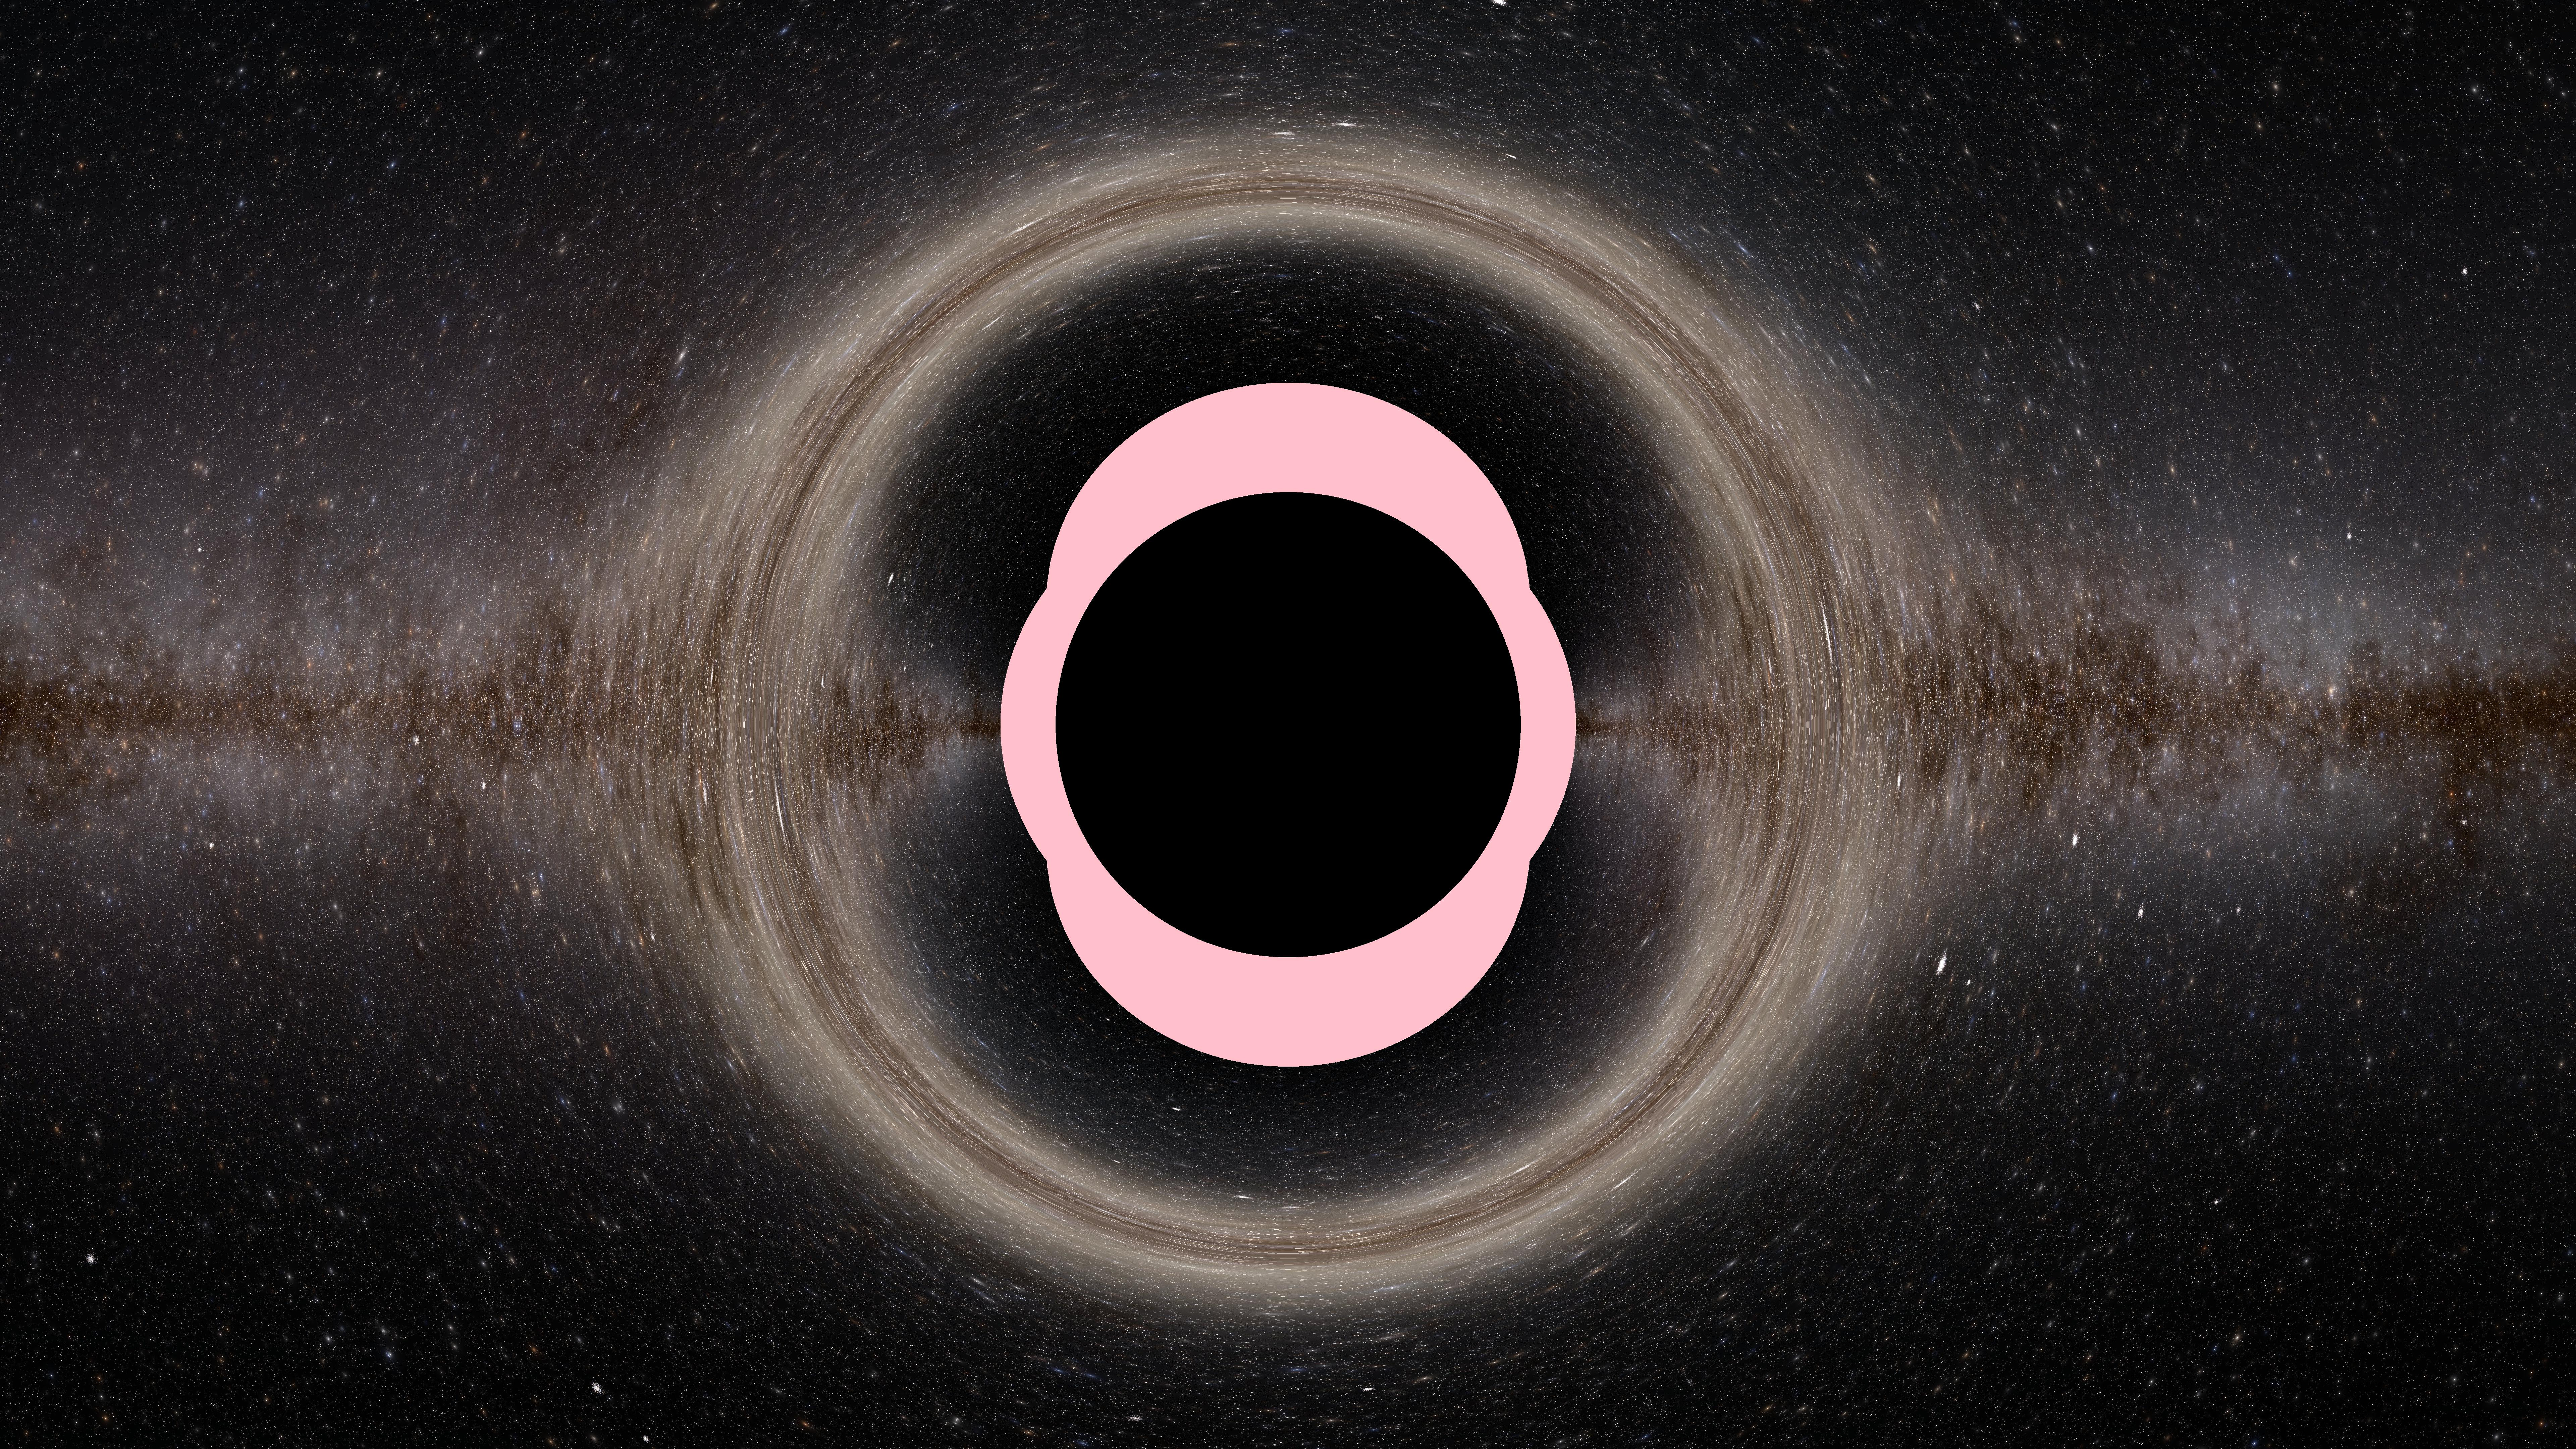
\includegraphics[width=0.8\linewidth]{img/8kstarfield-special}
	\caption{A model highlighting areas affected by the limited size of the image}
\end{figure}
\section{Analysing the image}

	Now that we have a high quality model for the effects of gravitational lensing caused by the Schwarzschild metric on a celestial sphere, we can take a look at the image and note some key features.

\begin{figure}[!ht]
	\centering
	\includegraphics[width=0.8\linewidth]{img/milkyway-SC}
	\caption{A model of a Schwarzschild black hole using a HDRI image, cropped.}
\end{figure}

	First, we note the purpose of using a HDRI image, and see the circular nature of the shadow caused by the event horizon, this stands to reason and is what we expect to see. 

\vspace{1em}
	The shadow can often be called the event horizon, but this is a misleading name, as it is really a shadow caused by photons being absorbed by the event horizon. This is a subtle distinction but the front side of the event horizon only takes up about half the area of the shadow, the rest is caused by photon paths which hit the back of the event horizon - or event orbit the black hole an amount of times and then hit the horizon. Naturally we can fine-tune the angle we fire a photon at and make a photon orbit the black hole and arbitrary amount of times - so the shadow is actually an image of an infinite number of copies of all faces of the event horizon.

\vspace{1em}
	The above description would be correct if the image was perfectly high definition, but due to image size there is a maximal number of orbits we can make a photon orbit, namely caused by the final layer of black pixels forming the shadow.

\vspace{1em}
	As circled in the image, we see that there are multiple images of notable features, including the star circled. This is due to the multiple paths photons may take to reach a point in space in the Schwarzschild metric; unlike in ordinary spacetime, where photons travel in near straight-lines, photon paths are 'bent' sufficiently in a black holes gravitational field that a photon may travel above and around a black hole to reach a point in space which may be reached by being bent slightly travelling below the black hole to begin with. This is specifically the case for the circled image; the primary image, caused by a photon travelling as directly as it can to the light source, is named as such as it is brighter and larger. The secondary image however requires a more conveluded path, above and around the black hole, so less photons may reach the light source via this route, leading to a smaller and less bright image.

\vspace{1em}
	This phenomenom may be seen for every light source on the original HDRI image acting as our celestial sphere, and not only that, if we had a high enough definition image, we would see tertiary images and so on infinitely as we zoom in on the outer layer of the shadow. These images would become thinner and less intense as we move closer due to the fact that we are requiring photons to orbit the black hole more times each image further we go.

\vspace{1em}
	We see that in a circle around the centre of the shadow, an image is formed from one same light source, this is because whatever lightsource lies directly behind the black hole in line with the camera has a circular primary image. Another way of thinking about this is that the shortest path to the point on the celestial sphere directly behind the black hole is to be bent back down to this line by the black hole, and since we have spherical symmetry, this angle is the same for whichever inclination we choose, as an interesting aside, this angle happens to be the y-axis intersection of the relation graph between $\alpha$ and $\alpha^{'}$. The image caused by this is named the Einstein ring of the black hole, and due to the celestial sphere chosen for Figure 4.6 is very notable.



\chapter{Kerr black holes}

	In this section I will move on to more general black holes, specifically ones with non-zero spin, I will introduce the Kerr metric and take a look at the equations of motions derived from the geodesic equation of light in the Kerr metric.

\section{The Kerr metric}

	The Kerr metric is used to describe a non-charged, rotating mass; often a black hole.

	 A Kerr black hole has spin parameter per unit mass J = $\frac{a}{M}$, where M is the mass of the black hole and a is a the spin parameter. J can range from 0 (describing a Schwarzschild black hole) to 1 (an extreme Kerr black hole). When J is taken to be greater than one, the Kerr metric can be used to describe a naked singularity, which is a singularity with no event horizon surrounding it.

	The Kerr metric of a mass M rotating with angular momentum a is given in line element by \cite{raquepas2017topics}:

	\[{ds^{2} = -\frac{\Delta}{\Sigma}(dt-a\mbox{Sin}^2(\theta)d\varphi)^2+\frac{\mbox{Sin}^2(\theta)}{\Sigma}((r^2+a^2)d\varphi-adt)^2)+\frac{\Sigma}{\Delta}dr^2+\Sigma d\theta^2}\]

\vspace{1em}
	With:
	
	\[\Delta(r) := r^2 - 2r + a^2\]
	\[\Sigma(r, \theta) := r^2 +(a\mbox{Cos}(\theta))^2\]

\section{Coordinate systems}

	There are two commonly used coordinate systems to formulate the Kerr metric in; Boyer-Lindquist coordinates\cite{boyer1967maximal} and Kerr-Schild coordinates\cite{debney1969solutions}. In section 5.1, we used Boyer-Lindquist coordinates, which are a form of 'stretched' spherical polar coordinates related to Euclidean spacetime by:

	\[t=t\]
	\[x = \sqrt{r^2+a^2}\mbox{Sin}(\theta)\mbox{Cos}(\varphi)\]
	\[y = \sqrt{r^2+a^2}\mbox{Sin}(\theta)\mbox{Sin}(\varphi)\]
	\[z = r\mbox{Cos}(\theta)\]

\vspace{1em}
	Take note that as is the case in many coordinate systems, there are areas which are ill defined in Boyer-Lindquist coordinates - namely when $\theta = 0\mbox{ or }\pi$, which corresponds to the z axis in three dimensional Euclidean space. A solution to this is to shift to a rotated Boyer-Lindquist system for any photon path which passes through I'll defined points. By 'stitching' these two coordinate systems together we avoid any problems. A quicker fix would be to discount any photon paths which pass through this line as there are very few of them.

\vspace{1em}
	Although less commonly used, the Kerr metric was proposed in 1965; two years after Kerr first formulated it, in Kerr-Schild coordinates. These are coordinates used to describe linear pertubations to spacetime metrics, and are a set of Cartesian coordinates, in the case of the Kerr metric given by:

	\[g_{\mu\nu} = \eta_{\mu\nu} + \frac{2r^{3}k_{\mu}k_{\nu}}{r^{4}+a^{2}z^{2}}\]
	\[\textbf{k} = (k_x,k_y,k_z) = \left(\frac{rx+ay}{r^2+a^2},\frac{ry-ax}{r^2+a^2},\frac{z}{r}\right)\]
	\[k_0 = 1\]

\vspace{1em}
	Generally Boyer-Lindquist coordinates are a more helpful coordinate system to work in, especially when looking at photon paths, but Kerr-Schild coordinates does have its advantages, notably the fact that the determinant of the metric tensor is equal to -1 everywhere in the metric.

\vspace{1em}
	Another coordinate system which is growing more popular in recent years is Doran coordinates\cite{doran2000new}. Designed such that as one tends angular momentum towards 0, Doran coordinates collapse to Painlev\'e–Gullstrand coordinates\cite{painleve1921mecanique} describing the Schwarzschild metric. The Kerr metric in line element in Doran coordinates by:

	\[ds^2=-dt^2+(r^2+a^2\mbox{Cos}^2(\theta))d\theta^2+(r^2+a^2)\mbox{Sin}^2(\theta)d\varphi^2+\]
	\[\left(\frac{r^2+a^2\mbox{Cos}^2(\theta)}{r^2+a^2}\right)\left\{dr+\frac{\sqrt{2Mr(r^2+a^2)}}{r^2+a^2\mbox{Cos}^2(\theta)}(dr-a\mbox{Sin}^2(\theta)d\varphi)\right\}^2\]

\vspace{1em}
	Some useful features include the fact that as we tend M to 0, the metric becomes the flat Minkowski metric in oblate spheriodal coordinates. Also, recalling notation for the inverse of the metric matrix; $g^{tt}=-1$ everywhere in Doran coordinates.

\vspace{1em}
	As mentioned in Section 3.2, as well as defining which coordinates we are using for the metric, we will also define which coordinate system we use for our camera; and consequentially how its frame of reference acts. 

\vspace{1em}
	We will be modelling the camera as a fiducial observer, a locally non-rotating observer. Crucially, a frame of reference which is at rest in Boyer-Linquist coordinates is not a fiducial observer, so although our camera is locally non-rotating, it is not at rest. It is also common to model a camera as actively orbitting the black hole for a more realistic image, this is prudent in the generation of animations; which this paper does not cover.

\vspace{1em}
	We will use spherical polar coordinates for our cameras frame of reference, though for calculation of angles, which includes launch and inclination angle I convert into Euclidean coordinates for more familiarity.

\vspace{1em}
	These considerations only apply as our camera is close enough to the metric to be affected by its spin, it is possible to have an observer far enough from the black hole for there to be no real difference between a fiducial observer and an observer at rest in Boyer-Lindquist coordinates. I choose to take these considerations into account as they allow me to better understand and communicate effects such as frame dragging (see Section 5.3) and relativistic abberation (see Section 6.4)

\section{Frame dragging}

	To have an inertial frame of reference, one usually alters the metric to have a co-rotating framework. This is an application of the Lense-Thirring effect, or rotational frame-dragging. In essense the Lense-Thirring effect is an effect caused by a rotating body which is rotating at such a speed that it is 'dragging' the matter around it and giving it angular momentum. The Lense-Thirring effect is the effect that has on an observer - or object we are interested in caused by this. This means that in extreme cases, it is not possible to stay stationary, regardless of momenta.

\vspace{1em}
	The Kerr metric is given most generally by:

	\[c^2d\tau^2 = g_{tt}dt^2+g_{rr}dr^2+g_{\theta\theta}d\theta^2+g_{\varphi\varphi}d\varphi^2\]

\vspace{1em}
	This can be rewritten as \cite{kerrMetric} to give an inertial frame of reference:

	\[c^2d\tau^2 = \left(g_{tt}-\frac{{g_{t\varphi}}^2}{g_{\varphi\varphi}}\right)dt^2+g_{rr}dr^2+g_{\theta\theta}d\theta^2+g_{\varphi\varphi}\left(d\varphi+\frac{g_{t\varphi}}{g_{\varphi\varphi}}dt\right)^2\]

\vspace{1em}
	This metric gives us a co-rotating reference frame, which is rotating with angular speed:

	\[\Omega = -\frac{g_{t\varphi}}{g_{\varphi\varphi}}\]

\vspace{1em}
	$\Omega$ is named the Killing horizon, and is relevant in section 5.4.

\vspace{1em}
	A commonly used analogy to explain frame dragging is that of a ballerina orbiting in the equatorial plane of a rotating black hole. This ballerinas frame of reference is stationary with respect to her celestial sphere, but is affected by frame dragging. To exemplify this, if the bellerina extends her arms outwards - one towards the centre of the black hole, and the other in the opposite direction, the parts of her frame closest to the black hole are given more angular momentum that the furthest. This causes her entire frame of reference to begin to rotate about the axis from her head to her toes (see Figure 5.1).

\vspace{1em}
	\begin{figure}[!ht]
	\centering
	\begin{minipage}{0.5\textwidth}
		\centering
		\includegraphics[width=0.8\linewidth]{img/addison-wesley}
		\caption{A model to help show the frame dragging effect. (Credit for figure skater image: Addison Wesley}
	\end{minipage}%
	\hfill
	\begin{minipage}{0.5\textwidth}
		\centering
		\includegraphics[width=0.8\linewidth]{img/Kerr-surfaces}
		\caption{A diagram showing key regions and surfaces in the Kerr metric \cite{yukterezkerrnewman}}
	\end{minipage}
\end{figure}

\section{Different regions of the metric}

	For a Schwarzschild black hole - the event horizon, the point at which we discard photon paths if crossed, is very simple. In fact it was theorised by Laplace as it is the natural limit using escape velocity in Newtonian physics. The escape velocity v for a particle on the surface of a body of mass M and radius R is given by:

	\[\frac{1}{2}v^2 = \frac{GM}{R}\]

\vspace{1em}
	When we set v = c for a photon we see that:

	\[R = \frac{2GM}{c^2} = 2M \mbox{ In natural units}\]

\vspace{1em}
	Which just so happens to be the Schwarzschild radius - the event horizon of a Schwarzschild black hole.

\vspace{1em}
	For a Kerr black hole the situation is a bit more complex, while there is still an event horizon, generated at the points in space for which $g_{rr}$ tends to infinity. Solving $\frac{1}{g_{rr}} = 0$ one finds that this horizon is located at \cite{kerrMetric}:

	\[{r_{H}}^{\pm} = 1\pm\sqrt{1+a^2}\]

\vspace{1em}
	Due to the rotation of a Kerr black hole, a region called the ergosphere (from the Greek word 'ergon' - meaning work) exists just outside the event horizon - This is a region which has 'requirements' to exist in, and is generated by the changing of sign of $g_{tt}$, the solely time dependant component of the Kerr metric, solving $g_{tt} = 0$ we see that the ergosphere lies at \cite{kerrMetric}:

	\[{r_{E}}^{\pm} = 1\pm\sqrt{1-a^2\mbox{Cos}^2(\theta)}\]

\vspace{1em}
	Inside this ergosphere - the space between the two above boundaries - $g_{tt}$ is negative. This means that a null geodesic entering the ergosphere changes from being light-like to space-like unless such an object is co-rotating with the black hole at sufficient speeds.

\vspace{1em}
	However, a null geodesic is by definition light-like, and so cannot be space-like. This means that the only possibility for light to enter the ergosphere is to co-rotate with the black hole with minimum angular speed $\Omega$.

\vspace{1em}
	Light-like curves can describe the paths of light-like objects inside a metric, whereas space-like curves can describe physical parameters, for example the length of an object.

\vspace{1em}
	However if a photon does in fact enter this ergosphere it has not yet passed the black holes event horizon, and so it is possible for it to escape. Furthermore as the photon enters the ergosphere it is forced to co-rotate and gain more energy. This energy is aquired from the black holes angular momentum, clearly if photons enter and exit the ergoregion the black hole loses angular momentum, and so theoretically energy can be harnessed from a rotating black hole. This process is called the Penrose-process, and is named after the British mathematician Roger Penrose who proposed it originally.

\vspace{1em}
	In Kerr-Schild coordinates, the Kerr metric is non-singular everwhere apart from the ring

	\[z=0\mbox{, } x^2+y^2=a^2\]

\vspace{1em}
	We see that using the Newman-Penrose formalism as in \cite{kerr2008discovering}, this is not just a coordinate singularity, but a singularity associated with the metric. Physically, this ring singularity is due to the fact that a mass formed from the collapse of a rotating fluid like matter (a star in most cases) will end up having a ring, rather than point, singularity. A non-rotating body collapsing will lead to just a point singularity, but due to the distribution of fluid-like matter when it rotates, the collapse of such a body will collapse down to a ring shaped singularity.

\vspace{1em}
	The Newman-Penrose (NP) formalism is a notation framework using spinor notation when working in a general reletivistic setting. Spinors are complex vectors associated with Euclidean space,  when the space is continuously rotated from 0 to 2$\pi$ radians, spinors are taken to the negative multiple of themselves. The NP formalism is based on, and is a subsection of the tetrad formalism, in which each tensor is projected onto a complete vector basis for each point in spacetime.

\vspace{1em}
	In a black hole with a point singularity, all test particles which enter the event horizon will end their path at the singularity. However; in the case of the Kerr metric, one can construct a path for a test particle such that it passes through the ring singularity, if this occurs then the metric changes, with r changing sign. What this means is that the Kerr metric can be used to model a kind of wormhole, as passing through the ring singularity takes a test particle to a different 'asymptotically flat' universe. This space is usually considered to be not physical but purely mathematical, and can be seen as a flat Minkawski space.

\chapter{Modelling photon paths in the Kerr metric}

	We take a more general backwards ray tracing approach to modelling a Kerr black hole, since the metric lacks spherical symmetry (meaning we cannot generalise to two dimensions), the interpolation method is significantly less efficient. As mentioned in section 3.6 this method, although slower, has it's upsides - notably freedom of initial lanch conditions.
	
\vspace{1em}
	Therefore we instead see our background image as a field of view, and for each pixel on the image, we calculate the required launch angle and inclination angle for a photon to reach this lightsource in ordinary spacetime. We then see where the modelled photon ends up and calculate the related pixel on a HDRI image.

\section{Deriving the equations of motion in the Kerr metric}

	There are many formulations of the equations of motion of a particle/photon in the Kerr metric, a notable difference in complexity appears compared to those derived from the Schwarzschild metric in section 3.2; this is because unlike the spherical symmertric we enjoy when working in the Schwarzschild metric, we now work in a metric with symmetry only about the axis of rotation. This symmetry does not symplify equations of motion much so we end up with the following, based upon \cite{yukterezKerr}:

\vspace{1em}
	Given initial position $(r, \theta, \varphi)$, initial velocity v, spin parameter a, launch angle $\alpha$ and inclination angle $\delta$ one may use Hamiltonians formalism on the Kerr metric to find:
	
	\[v_r = v\mbox{Sin}(\alpha), v_\varphi = v\mbox{Cos}(\alpha)\mbox{Sin}(\delta), v_\theta = v\mbox{Cos}(\alpha)\mbox{Cos}(\delta)\]

\vspace{1em}
	For ease of notation, along with $\Sigma$ and $\Delta$, I define $\chi$ as follows:

	\[\chi = (r^2+a^2)^2-a^2\mbox{Sin}^2(\theta)\Delta\]

\vspace{1em}
	Then for our calculable initial conditions and constants:

	\[\omega = \frac{2ar}{\chi}\]
	\[L_{z} = v_{\varphi}\mbox{Sin}(\theta)\sqrt{\frac{\chi}{\Sigma}}\]
	\[ E = L_{z}\omega\]
	\[p_{\varphi} = L_{z}\]
	\[p_{r} = v_{r}\sqrt{\frac{\Sigma}{\Delta}}\]
	\[p_{\theta} = v_{\theta}\sqrt{\Sigma}\]
	\[Q = {p_{\theta}}^2+\mbox{Cos}^2(\theta)\left(\frac{{L_{z}}^2}{\mbox{Sin}^2(\theta)}-a^2E^2\right)\]
	\[k = Q+{L_{z}}^2+a^2E^2\]

\vspace{1em}
	And for our system of first order differential equations:

	\[\dot{r} = p_r\frac{\Delta}{\Sigma}\]
	\[\dot{\theta} = \frac{p_\theta}{\Sigma}\]
	\[\dot{\varphi} = \frac{2arE+L_{z}\mbox{Cosec}^2(\theta)(\Sigma-2t)}{\Sigma\Delta}\]
	\[\dot{p_{\varphi}} = 0\]
	\[\dot{p_{\theta}} = \frac{\mbox{Sin}(\theta)\mbox{Cos}(\theta)(L^2\mbox{Cosec}^4(\theta)-a^2E^2)}{\Sigma\Delta}\]
	\[\dot{p_{r}} = \frac{2rE^2(r^2+a^2)-k(r-1)-2aEL_{z}}{\Sigma\Delta}-\frac{2{p_{r}}^2(r-1)}{\Sigma}\]

\section{Modelling a photon path}

	As mentioned above, we will be modelling the path of a photon in the Kerr metric using reletivistic ray tracing. We will be using solve\_ivp and running along a time related variable $\tau$, in the equations shown in section 6.1 a differentiation with respect to this variable is denoted using a dot. Since we are not planning on creating an animation in this paper the relationship between $\tau$ and t does not affect our final image; only that $\tau$ runs over an appropriate range.

\vspace{1em}
	Running along this basis we use solve\_ivp to generate a list of $r,\theta,\varphi,p_{\varphi},p_{\theta},p_{r}$ and from this we can plot the path of such a photon using Boyer-Lindquist coordinates (See Figure 6.1).

\vspace{1em}
	The first thing we will do is to find our launch angle and inclination angle for given pixel (i,j) on a HDRI image. By construction a HDRI image is 2x1 aspect ratio and the (i,j) pixel corresponds to angles x,y rotation about the y-z,x-z plane respecitvely. A simpler way to think of this is that i is directly proportional to $\theta$, and j to $\varphi$ in the usual three dimensional polar coordinates (here with r = celestial sphere radius).

\vspace{1em}
	Via some elementary geometry, we see that our launch angle $\alpha$ - the angle formed at the tangent at our initial position with the x-axis, and the inclination angle $\delta$ - the angle required to rotate about the x-axis to form our tangent, are:

	\[\alpha = \mbox{Cos}^{-1}(\mbox{Cos}(x)\mbox{Cos}(y))\]
	\[\delta = \mbox{Tan}^{-1}\left(\frac{\mbox{Sin}(y)}{\mbox{Sin}(x)\mbox{Cos}(y)}\right)\mbox{ If i}>0\mbox{ and} \]
	\[\delta = \pi+\mbox{Tan}^{-1}\left(\frac{\mbox{Sin}(y)}{\mbox{Sin}(x)\mbox{Cos}(y)}\right)\mbox{ If i}<0\]

\vspace{1em}
	A special case arises if i=0, due to the coordinate system mentioned in section 5.2. Here I take inclination angle to be $0,\pi$ when j is positive and negative respectively.

\begin{figure}[!ht]
	\centering
	\includegraphics[width=0.4\linewidth]{img/3d-kerr-plot}
	\caption{A plot of a photon in the Kerr metric (r=3,$\theta=\frac{\pi}{2}$,$\varphi$=0,v=1,a=1,$\alpha$=0,$\delta$=-$\mbox{Arcsin}(\frac{1}{3})$}
\end{figure}

\section{Generating an image}

	After we have this, for each pixel in our image, we numerically solve the coupled differential equations governing the equations of motion using our initial conditions and keep a list of relevant variables across a time basis. If the solution status shows that an event took place  (i.e the photon passed the event horizon), we update the current pixel to black on a copy of our celestial sphere image. If not, we find the final point ($x_1,y_1,z_1$) of our photons path in x,y,z coordinates and find the angles formed with a straight line from our initial position ($x_0,y_0,z_0$) to final position with the x-z plane and the x-y plane for a tuple directly proportional to the pixel coordinates of the final position on the original image.

\vspace{1em}
	Again, via elementary geometry, one can find:

	\[\theta_{x} = \mbox{Tan}^{-1}\left(\frac{x_1-x_0}{y_1-y_0}\right)\]
	\[\theta_{y} = \mbox{Tan}^{-1}\left(\frac{z_1-z_0}{\sqrt{(x_1-x_0)^2+(y_1-y_0)^2}}\right)\]

\vspace{1em}
	This is just for one sector of final positions, for others signs change and constants are added.

\vspace{1em}
	After converting these angles to pixel coordinates, and updating our copy of the celestial sphere with the relevant final pixel position, we get an image like Figure 6.2.

\begin{figure}[!ht]
	\centering
	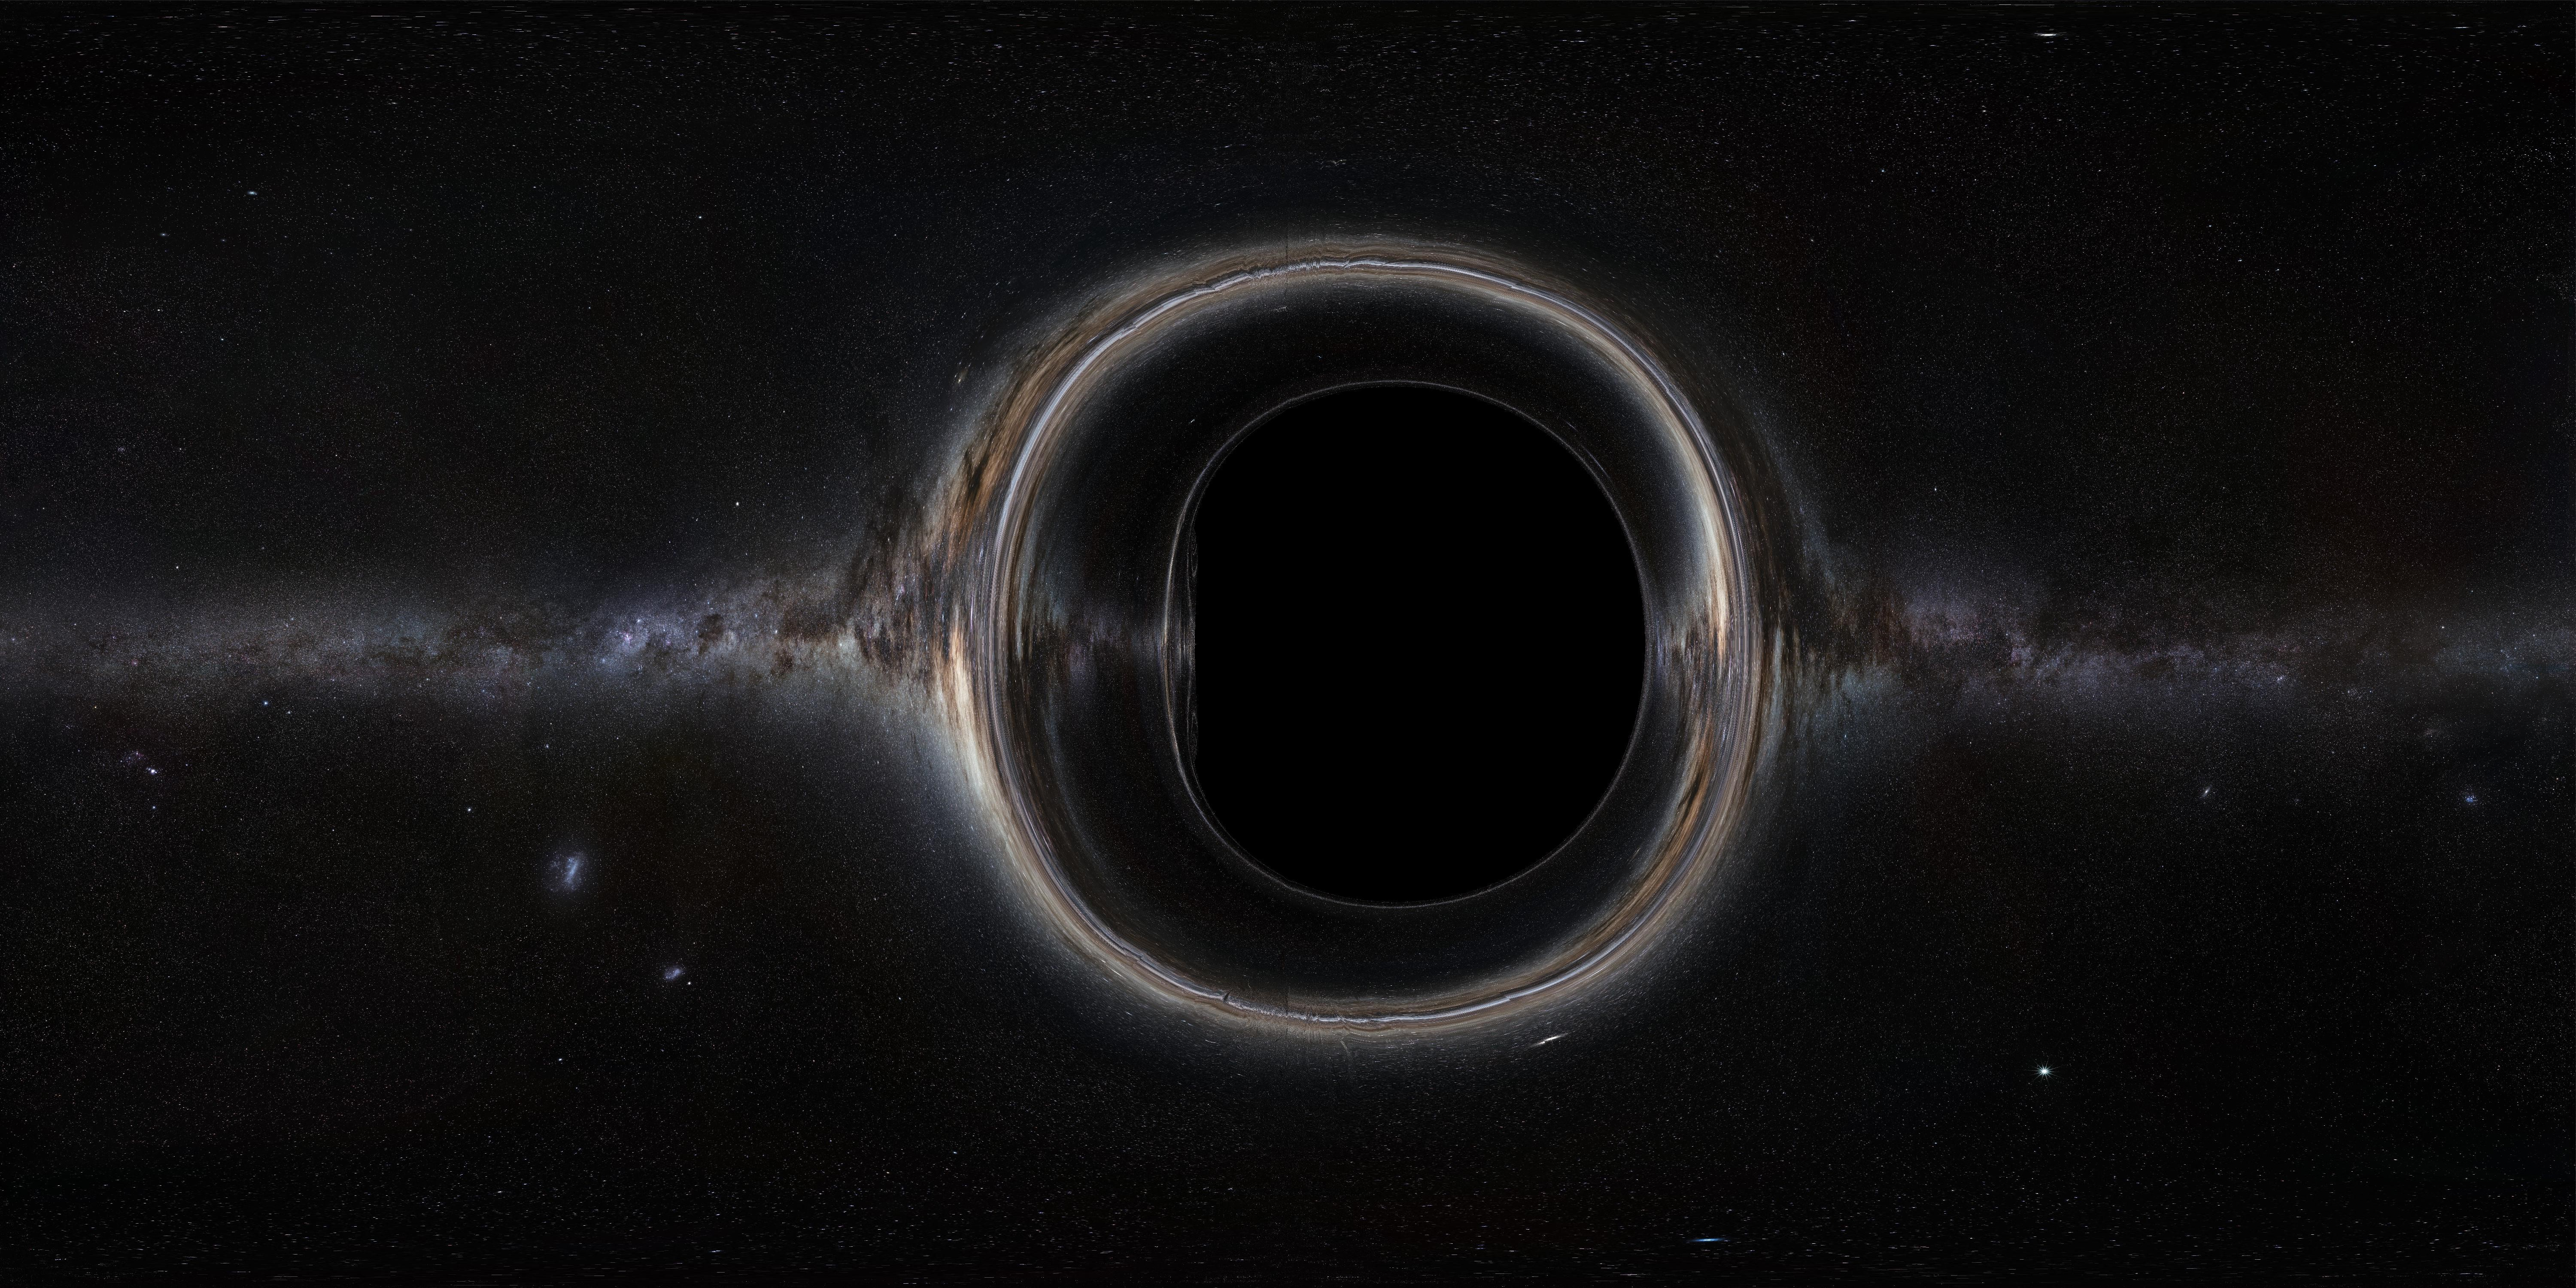
\includegraphics[width=\linewidth]{img/milkyway-kerr-full-new}
	\caption{A model of a Kerr black hole with spin parameter a=0.998}
\end{figure}

\section{Analysing the results}

	Looking carefully at Figure 6.2, we can see some very interesting and telling things which inform us of the nature of the Kerr metric. 

\vspace{1em}
	First and foremost is the event horizon, as mentioned in chapter 1, we see the distinctive D-shape event horizon. The transformation from central and circular to this shape is smooth, as one would expect, as spin parameter increases. This shape comes from the fact that a photon orbiting the black hole in the same direction as it's spin gains energy - and conversely a photon orbiting against the direction of spin loses energy, so where a photon in the Schwarzschild metric may cross the event horizon; if it is corotating with a Kerr black hole it may escape.

\vspace{1em}
	As was the case with the images we generated of the gravitational lensing caused by a Schwarzschild black hole, we can see various repeated images - with a particularly notable example near the flat edge of the shadow. The explaination as to the primary, secondary and so on images given in section 4.6 remains applicable in the Kerr metric, and the reasoning behind the clear example on the flat side is due to how close we are able to approach the event horizon and escape. 

\vspace{1em}
	There are very few pixels relating to retrograde paths (non co-rotating) which allow for multiple orbits and eventual escape of the black hole, given a perfect image and zooming capabilities we would still see an infinitely repeating pattern, though interestingly a very different pattern to those produced by prograde orbits (see \cite{riazuelo2012some}). However, on the opposite side of the picture, with pixels relating to prograde paths, there is a significantly larger area in which photons may orbit the black hole many times and escape due to the gained angular momentum.

\vspace{1em}
	Much of the repeating images on the flat side are caused by photon orbits which enter and exit the ergoregion; this is extreme due to the extremity of the spin parameter used, making the possible energy gained, and maximal distance between outer horizon and outer ergosphere very large.

\vspace{1em}
	The size of the shadow is affected by relativistic abberation; an effect in special and general relativity caused by the speed of an observer. If an observer is moving at a considerable fraction of the speed of light, the captured image is very different to that of an observer at rest. Since we take a fiducial observer, which is not at rest, our image is representative only of an observer at rest rotationally. The more one corotates with a Kerr black hole, the less of it's shadow one will see, meaning a totally at rest observer would see more of the black holes shadow.


\section{Caustics and critical curves}

\vspace{1em}
	As in the case of the image relating to the Schwarzschild metric, we see critical curves - an analogue to the Einstein ring; formed due to all photon paths ending on the primary caustic of the image. This primary caustic is the intersection between a caustic line on the cameras past light-cone and the celestial sphere. Rather than a point directly behind the black holes centre in line with the camera as is the case in the Schwarzschild metric, this primary caustic is a small closed curve. The primary critical curve is not circular; but rather a rounded rectangular shape, and can be clearly seen in Figure 6.2.

\vspace{1em}
	The secondary critical curve is the exactly the same as the primary critical curve but it is generated by the secondary caustic. Each time you 'cross' a critical curve the direction of motion of the image flips, meaning that there are divergent shears at each critical curve.

\vspace{1em}
	It can be difficult to visualise without animation but as mentioned above, if we were to produce an animation from an orbitting camera we would see that the direction of motion for stars on the image switches each time we cross a critical curve.

\vspace{1em}
	Critical curves cause some very interesting behaviour, including the creation and annahilation of stellar image pairs; as a stars position on our celestial sphere changes, it may cross a critical curve. Since critical curves are closed and due to the nature of a natural orbit, this path must also take the star out of the critical curve at some point. Each time a star crosses a critical curve a stellar image pair is either created or annihilated; what this means is that two new images of the star will either be formed, or destroyed. 

\vspace{1em}
	At the moment of creation, the relative intensity of the stars new images spikes dramatically, causing creation and annihilation to be noticable in animations \cite{}.

\section{Testing Accuracy}

	To check that my generated image is correct, I ran my code for a well known and understood celestial sphere; a checkerboard of paint. This also serves to provide a very clear picture to show how the gravitational lensing affects the original image, as each final section can be traced to its origins on the original picture.

\vspace{1em}
	\begin{figure}[!ht]
	\centering
	\begin{minipage}{0.5\textwidth}
		\centering
		\includegraphics[width=0.8\linewidth]{img/checkerboard}
	\end{minipage}%
	\hfill
	\begin{minipage}{0.5\textwidth}
		\centering
		\includegraphics[width=0.8\linewidth]{img/checkerboard-kerr}
	\end{minipage}
	\caption{A model showing the effects of gravitational lensing on a coloured checkerboard. (Credit for original image to DNEG)}
\end{figure}

\vspace{1em}
	The result of this test was an almost one-to-one image, which shows my code is running well, at least on a cursory glace. Rather unsurprisingly we see that the more central a colour is, the more space it takes up in the final image, this is because there are many relatively 'easy' paths a photon can take to reach more central colours.

\chapter{Realism and beyond}

	Now that we have an accurate model of the gravitational lensing caused by a Kerr black hole we can begin to consider effects and properties to improve the realism of our currently idealised model.

\section{Accretion disc}

	Given what we know of black holes in the universe, in all likelihood most if not all active black holes are surrounded by matter which orbits the singularity and 'feeds' the black hole. This matter is known as an accretion disc, and there are various methods one can use to model them.

\vspace{1em}
	The simplest model for an accretion disc is a flat annulus on the equatorial plane of the black hole, we can keep track of if a photon path intersects with this annulus and if so use a png to map the final pixel to launch pixel. This is the most common but unrealistic method of modelling, and gives us a good general idea as to what an accretion disc looks like from an observers standpoint. This kind of model can be used to form an image similar to Figure 6.3, with a test accretion disc to show explicitly what the effects of gravitational lensing on an accretion disc are (see Figure 7.1)

\vspace{1em}
	A much more realistic method is to model the accretion disc as a gas-like energy with an accretion rate which affects the energy flux. This is a thin relativistic accretion disc and the effects covered in section 7.2 can be easily applied. Interestingly the first, 'simple', approach is a good approximation to this method when taking the disc not to be accreting energy, as was the model for the film Interstellar. This method was used by Jean-Pierre Luminet to find apparent bolometric flux at various radii around a Kerr black hole and create the first 'image' of an accretion disc based upon mathematics.

\vspace{1em}
	Assuming we have positive spin (we can do this using the axial symmetry of the Kerr metric) we may model the intrinsic flux of an accretion disc as:

\vspace{1em}
\begin{dmath}
\mbox{F}_s = \frac{3\dot{\mbox{M}}_0}{8r\pi(r^{\frac{3}{2}}-3r^{\frac{1}{2}}+2a)}\left(r^{\frac{1}{2}}-x_0-\frac{3a}{2}\mbox{log}\left(\frac{r^{\frac{1}{2}}}{x_0}\right)-\frac{3(x_1-a)^2}{x_1(x_1-x_2)(x_1-x_3)}\mbox{log}\left(\frac{r^{\frac{1}{2}}-x_1}{x_0-x_1}\right)-\frac{3(x_2-a)^2}{x_2(x_2-x_1)(x_2-x_3)}\mbox{log}\left(\frac{r^{\frac{1}{2}}-x_2}{x_0-x_2}\right)-\frac{3(x_3-a)^2}{x_3(x_3-x_1)(x_3-x_2)}\mbox{log}\left(\frac{r^{\frac{1}{2}}-x_3}{x_0-x_3}\right)\right)
\end{dmath}

\vspace{1em}
 With

\[a = \mbox{positive spin}\]
\[Z_1 = 1+(1-a^2)^{\frac{1}{3}}\left((1+a)^{\frac{1}{3}}+(1-a)^{\frac{1}{3}}\right)\]
\[Z_2 = (3a^2+{Z_1}^2)^{\frac{1}{2}}\]
\[x_0 = (3+Z_2-\left((3-Z_1)(3+Z_1+2Z_2))^{\frac{1}{2}}\right)^{\frac{1}{2}}\]
\[x_1 = 2\mbox{Cos}(\frac{1}{3}\mbox{Cos}^{-1}(a)-\frac{\pi}{3}), x_2 =2\mbox{Cos}(\frac{1}{3}\mbox{Cos}^{-1}(a)+\frac{\pi}{3}) , x_3 = -2\mbox{Cos}(\frac{1}{3}\mbox{Cos}^{-1}(a))\]

\vspace{1em}
	Now apparent bolometric flux (the flux at an observer) can be written as

\[\mbox{F}_0 = \frac{\mbox{F}_s}{(1+z)^4}\]

\vspace{1em}
	Taking this a step further, in Astrophysics of Black Holes\cite[pg.435-439]{} Thorne and Novikov took the $\alpha$-disc model by Shakura and Sunyaev\cite{} and took into account relativistic effects to create an explicit formulation of an accretion disc consisting of an inner, middle and outer region

\section{Relativistic Doppler shift and abberation}

\section{Falling into a black hole}

\appendix
%\include{appendix1}
%\include{appendix2}

%\nocite{}
\bibliographystyle{ieeetr}
\bibliography{bibliography}{}
\end{document}